
\documentclass[a4paper,12pt,oneside]{book}

%-----------------------
%PACKAGES
%-----------------------


\usepackage[DIV=15,headinclude=true,footinclude=false]{typearea} %better layout
\usepackage{fullpage} % Package to use full page
\usepackage[table,xcdraw,dvipsnames]{xcolor} %meer kleurtjes
\usepackage{parskip} % Package to tweak paragraph skipping
\usepackage{tikz} % Package for drawing
\usepackage{amsmath} %display math
\usepackage{hyperref} %hyperlinks in text
\usepackage{listings} %show formatted python/r code
\usepackage{color} %duh
\usepackage[T1]{fontenc} %better fonts
\usepackage[bitstream-charter]{mathdesign} %math-text in text
\usepackage{ccicons} %creative commons license stuff
\usepackage[ddmmyyyy,hhmmss]{datetime}

\usepackage[page]{appendix} %appendix usage
\usepackage{fancyvrb} %for verbatim usage; no longer used in this document?
\usepackage{enumitem} %better control of lists
\usepackage{titlesec} %alternative section titles
\usepackage[activate={true,nocompatibility},final,tracking=true,kerning=true,spacing=true,factor=1100,stretch=10,shrink=10]{microtype} %beter fonts
\usepackage{pdfpages} %insert pdfs
\usepackage{siunitx}
\usepackage{fancyhdr}
\usepackage{background}
\usepackage{lastpage}

\usepackage[type={CC},modifier={by-nc},version={4.0}]{doclicense}

%----------------------
%SETUP
%----------------------

\renewcommand*\contentsname{Inhoud} %NL name for contents

%automatic studyyear calculation for front page
\newcommand\PrevYear{%
   \advance\year by -1 \the\year\advance\year by 1}

\newcommand\NextYear{%
   \advance\year by 1 \the\year\advance\year by -1}

\definecolor{saxion}{RGB}{0,150,120} %saxion-groen

%links
\hypersetup{
    colorlinks=true,
    linkcolor=saxion,
    filecolor=magenta,      
    urlcolor=saxion,
}

%colors for code display
\definecolor{codegreen}{rgb}{0,0.6,0}
\definecolor{codegray}{rgb}{0.5,0.5,0.5}
\definecolor{codepurple}{rgb}{0.58,0,0.82}
\definecolor{backcolour}{rgb}{0.95,0.95,0.92}

%code display settings
\lstdefinestyle{mystyle}{
    backgroundcolor=\color{backcolour},   
    commentstyle=\color{codegreen},
    keywordstyle=\color{magenta},
    numberstyle=\tiny\color{codegray},
    stringstyle=\color{codepurple},
    basicstyle=\footnotesize,
    breakatwhitespace=false,         
    breaklines=true,                 
    captionpos=b,                    
    keepspaces=true,                 
    numbers=none,                    
    numbersep=5pt,                  
    showspaces=false,                
    showstringspaces=false,
    showtabs=false,                  
    tabsize=2,
    upquote=true
    frame=single
}

% \lstinputlisting settings / always have frame
\let\oldlstinputlisting\lstinputlisting
\renewcommand{\lstinputlisting}[2][]{\oldlstinputlisting[frame=single]{#2}}
\lstset{basicstyle = \ttfamily,columns=fullflexible}

%chapter/section title settings
\titleformat{\chapter}{\normalfont\huge\color{saxion}}{\thechapter.}{20pt}{\huge}[\titlerule]
\titleformat{\section}{\normalfont\Large\color{saxion}}{\thesection.}{16pt}{\Large}[\titlerule]
\titleformat{\subsection}{\normalfont\large\color{saxion}}{\thesubsection.}{15pt}{\large}
\titleformat{\subsubsection}{\normalfont\color{saxion}}{\thesubsubsection.}{12pt}{\normalsize}

\backgroundsetup{contents={}}

 
%----------------------
%FRONT PAGE - not used
%----------------------




%\title{Dataverwerking \\ Studiewijzer en Dictaat }
%\author{Opleiding Chemie, Saxion Deventer en Enschede}
%\date{Leerjaar 2, kwartiel 2, studiejaar %\the\year/\NextYear{}}

%---------------------
%CONTENTS
%---------------------


\begin{document}

\lstset{language=r}
\lstset{style=mystyle}

\makeatletter
    \begin{titlepage}
	\centering
	\vspace*{1.5in}
	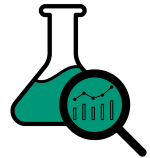
\includegraphics[]{img/logodata.png}\par\vspace{1cm}
	{\huge Dataverwerking \par}
	{\Large Studiewijzer en Dictaat\par}
	\vspace{1.5cm}
	{\large Opleiding Chemie\par}
	{\large Saxion Deventer en Enschede\par}


	\vfill
    \end{titlepage}
\makeatother
\thispagestyle{empty}
\newpage

\begin{center}

{\Large Colofon}\\
\vspace{15mm}

\includegraphics[width=0.7\linewidth]{img/lg_saxion_rgb.png}
\end{center}
\vspace{10mm}
Dit document is opgesteld door:\\
Karin Heutinck (\href{k.j.b.heutinck@saxion.nl}{\textsf{k.j.b.heutinck@saxion.nl}}) - Multivariate dataverwerking \& DoE\\
Taco Graafsma (\href{t.l.g.p.graafsma@saxion.nl}{\textsf{t.l.g.p.graafsma@saxion.nl}}) - Gegevensbeheer \\
Samuel Mok (\href{s.mok@saxion.nl}{\textsf{s.mok@saxion.nl}}) - Datamanagement\\
voor de opleiding Chemie van de Saxion Hogeschool ter behoeve van de leerlijn Dataverwerking in het jaar \the\year.

Met dank aan Sonja Scheinhardt voor een deel van het materiaal voor Design of Experiments.

Dit dictaat heeft een CC4-BY-NC licentie (zie hieronder). Dit dictaat is geschreven in de taal \LaTeX\ in de editor Overleaf en is hier beschikbaar: \href{https://www.overleaf.com/read/sgpyzkvsfkpc
}{overleaf.com}. De broncode is beschikbaar op de volgende GitHub repository: \href{https://github.com/MokSamuel/Studiewijzer-Dataverwerking}{https://github.com/MokSamuel/Studiewijzer-Dataverwerking}

Voor het laatst aangepast op \today.
\doclicenseThis


\tableofcontents


\setcounter{page}{1}
 \backgroundsetup{
  scale=1,
  color=black,
  opacity=1,
  angle=0,
  position=current page.south,
  vshift=60pt,
  contents={%
  \small\sffamily%
  \begin{minipage}{.8\textwidth}
  \parbox[b]{.6\textwidth}{%
    Dictaat Dataverwerking}\hfill
  \textcolor{saxion}{\rule{\textwidth}{1.5pt}}\\
  Opleiding Chemie - Saxion
  \end{minipage}\hspace{.02\textwidth}%
  \begin{minipage}{.18\textwidth}
  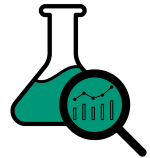
\includegraphics[width=\linewidth,height=70pt,keepaspectratio]{img/logodata.png}
  \end{minipage}%
  }
}


\chapter{Studiewijzer}

Dit dictaat bevat informatie voor het vak "Dataverwerking" wat wordt gegeven in het 2e en 3e kwartiel van het 2e jaar van de opleiding Chemie. Dit dictaat begint met een overzicht van dit onderdeel, het materiaal, de leerdoelen, en de vorm van toetsing en beoordeling. Vervolgens bevat dit document achtergrondinformatie en materiaal wat nodig is tijdens het uitvoeren van dit vak.


\section{Materiaal}
\label{sec:software}
Het materiaal wat je nodig hebt voor dit vak is beschikbaar op Blackboard in de module Chemical Fingerprinting. Hier vind je o.a. databases, voorbeeldbestanden, etcetera. 

Naast het materiaal wat er wordt aangeboden is er geen boek nodig voor dit vak. Wel heb je een laptop nodig met software. De software die wordt gebruikt in dit vak (installeer in ieder geval de eerste 3 voordat de lessen beginnen):
\begin{enumerate}
    \item Microsoft Office (Excel, Onedrive, Access): Downloaden op \href{https://office.com}{\textsf{office.com}}. Als je inlogt met je Saxion-account kan je gratis het complete office-pakket downloaden. Let op dat je de nieuwste versie van Office hebt, en dat je ingelogd bent op je Saxion-account! Deze software wordt gebruikt vanaf week 3. 
    \item R: R is een programmeertaal die zich richt op statistische bewerkingen. Dit gebruiken we het hele vak door. Je kan dit downloaden vanaf \href{https://cran.uni-muenster.de/}{\textsf{r-project.com}}.
    \item Blue Sky Statistics: Downloaden vanaf \href{https://www.blueskystatistics.com/}{\textsf{blueskystatistics.com}}. Dit softwarepakket is gratis te downloaden en wordt gebruikt vanaf week 1. 
    \item RStudio: Downloaden vanaf \href{https://rstudio.com/}{\textsf{rstudio.com}}. Dit softwarepakket is gratis te downloaden en wordt gebruikt vanaf week 7.
    \item Python: Dit wordt gebruikt in kwartiel 3, maar kan al goed van pas komen dit kwartiel! Je kan dit dus alvast installeren. Om dit (gratis) te downloaden kan je terecht op de Anaconda website \href{https://www.anaconda.com/distribution/}{anaconda.com}.
    \item (optioneel) SPSS: Dit is in leerjaar 1 gebruikt en kan worden gebruikt voor bepaalde analyses. Dit wordt echter niet aangeraden, en er is geen ondersteuning voor deze software in dit vak. SPSS kan je aanschaffen op \href{https://www.surfspot.nl/}{surfspot.nl}.
\end{enumerate}

\section{Leerdoelen}
De leerdoelen voor dit vak zijn algemeen geformuleerd en worden tijdens de lessen verder toegelicht.
\begin{itemize}
    \item Het kunnen uitvoeren en correct interpreteren van een multivariate clusteranalyse
    \item Het kunnen uitvoeren en correct interpreteren van een principale componentenanalyse
    \item Gegevens systematisch en gestructureerd op kunnen slaan aan de hand van een simpel datamanagementplan (DMP)
    \item Het begrijpen en kunnen toepassen van metadatadocumenten bij de opslag van data
    \item Het bewerken van verkregen gegevens voor langdurige opslag en mogelijke verdere verwerking
    \item Kennis verkrijgen over de werking van databases
    \item Het kunnen werken met een eenvoudige acces-database
    \item De basisprincipes van design of experiments begrijpen en kunnen toepassen
    \item Het kunnen opzetten van een 2\textsuperscript{n} factorial design

\end{itemize}

\section{Planning}

Iedere week komt er een ander onderwerp aan bod. Bij ieder onderwerp hoort een opdracht. Voor het overzicht is onderstaande tabel gemaakt:

\begin{table}[h]
\begin{tabular}{|l|l|l|}
\hline
\rowcolor{saxion}
Weeknummer & Onderwerp                    & Opdracht                         \\ \hline
1          & Datamanagementplan           & Opdracht DMP case                                  \\ \hline
2          & Importeren \& verwerken data & Verwerken in project kwartiel 2           \\ \hline
\rowcolor[HTML]{C0C0C0} 
3          & Clusteranalyse               &                                  \\ \hline
\rowcolor[HTML]{C0C0C0} 
4          & Principale Compentenanalyse  & Verwerken in project kwartiel 2 \\ \hline
5          & Databases 1                  &                                  \\ \hline
6          & Databases 2                  & Opdracht databases               \\ \hline
\rowcolor[HTML]{C0C0C0} 
7          & Design of Experiments 1      &                                  \\ \hline
\rowcolor[HTML]{C0C0C0} 
8          & Design of Experiments 2      & Verwerken in project kwartiel 3 \\ \hline
\end{tabular}
\end{table}


\section{Toetsing}

Dit vak wordt in meerdere onderdelen getoetst. In principe wordt er vanuit gegaan dat je vanaf nu de kennis van dit vak gebruikt waar nodig en/of zinvol. Een deel van het vak wordt getoetst in kwartiel 3 bij de eindopdracht dataverwerking (3 EC). De rest wordt getoets bij de praktijkopdrachten van kwartiel 2 en 3: bij het project chemical fingerprinting, urban mining, en met losse opdrachten bij professional skills 2. De details zijn te vinden op de Blackboardpagina's van de relevante kwartielen. Een kort overzicht van de onderdelen waarin dataverwerking terugkomt de komende kwartielen vind je in de tabel hieronder. Aan deze tabel kunnen geen rechten worden ontleend, het meest recente overzicht kan je altijd vinden op Blackboard onder het kopje Toetsinformatie.

\begin{table}[h]
\begin{tabular}{|l|l|l|}
\hline
\rowcolor{saxion} 
\textbf{Opdracht}       & \textbf{Onderdeel} & \textbf{Kwartiel} \\\hline
Werkplan                & Prof. Skills 2     & 2                 \\\hline
Onderzoeksstrategie     & Prof. Skills 2     & 2                 \\\hline
Eindverslag             & Prof. Skills 2     & 2                 \\\hline
Opdracht dataverwerking & Prof. Skills 2     & 2                 \\\hline
Werkplan                & Prof. Skills 3     & 3                 \\\hline
Verslag                 & Prof. Skills 3     & 3                 \\\hline
Eindopdracht data       & Losse toets (3 EC) & 3                 \\\hline
\end{tabular}
\end{table}


\chapter{Datamanagement}
\label{chap:datamanagement}
Deze lessen gaan over het importeren, opslaan, verwerken, en aanpassen van data voor later gebruik.

\section{Beheer van gegevens}
Of je nou analyses uitvoert, polymeren onderzoekt, nanotechnologisch bezig bent: als chemicus ben je constant bezig om data te verkrijgen, te verwerken, en te interpreteren. 

Een van de belangrijkste dingen hierbij is dat data systematisch wordt opgeslagen in een vorm die ook later nog bruikbaar is. De eerste les van dit onderdeel gaat hierover: welke technieken zijn er om je gegevens te beheren?

In dit onderdeel houden we het bij relatief simpele voorbeelden: gegevens die overzichtelijk in excel-sheets passen en die door 1 persoon worden beheerd en gebruikt. Voor meer ingewikkelde gevallen heb je vaak databases nodig, om bijvoorbeeld grote hoeveelheden data te beheren of om meerdere personen op verschillende manieren toegang te kunnen verlenen. Databases komen aan bod in hoofdstuk~\ref{chap:gegevensbeheer}: Gegevensbeheer.

Voor het opslaan van data maak je van tevoren een plan, die je eventueel aanpast indien nodig. Het maken van een datamanagentsplan (DMP) is verplicht in veel sectoren: onderzoekers moeten bijvoorbeeld zo'n plan aanleveren bij de aanvraag van onderzoeksgeld. Er zijn een heleboel manieren om een dergelijk plan te maken. In dit hoofdstuk wordt er 1 manier doorgewerkt. Het is de bedoeling dat jullie ook een DMP maken voor jullie project Chemical Fingerprinting (en later ook voor Urban Mining).

Een datamanagementsplan bestaat uit verschillende aspecten. Hieronder worden de mogelijke onderdelen besproken, en er wordt meer informatie gegeven over technische aspecten. Vervolgens zal je een voorbeeldcase uitgewerken. In Appendix~\ref{ap:dmp} staat een sjabloon voor het maken van een DMP. 
\begin{itemize}
    \item \textbf{Algemene info}: Het plan bevat een voorblad met de meest essentiële informatie. Denk hierbij aan deelnemers (personen en organisaties), tijdsduur, datum, titel project, taken en rollen van personen
    \item \textbf{Verzamelen}: welk type data wordt er gegenereerd, hoe wordt deze verkregen, in welk formaat, de geschatte grootte van de dataset, de geschatte kosten, en of alles binnen wetgeving valt
    \item \textbf{Documentatie}: in welk format wordt de data opgeslagen, moeten er nog extra documenten bij met uitleg en metadata, in wat voor structuur wordt het opgeslagen, hoe wordt versiebeheer geregeld 
    \item \textbf{Opslag}: wat moet er allemaal worden opgeslagen, waar wordt het opgeslagen, wat zijn de kosten
    \item \textbf{Veiligheid}: is er betrouwbare data bij, wie mag bij welke data, moet data worden opgesplitst in losse sets, wie is de eigenaar van de data, en wat gebeurt er mee na het onderzoek
    \item \textbf{Selectie en behoud}: moet de data voor langere termijn worden bewaard, wie is daar verantwoordelijk voor, hoe wordt dat geregeld, hoe lang moet het worden bewaard
    \item \textbf{Reproductie}: wie mag de data verder gebruiken, welke licentie zit er op de data
\end{itemize}

De meeste onderdelen spreken voor zich. De technische aspecten zijn voor veel van jullie nog nieuw, dus daar wordt wat extra aandacht aan besteed.

\subsection*{Opslag van data}
Als je je bestanden wil opslaan zijn er een boel dingen waar je rekening mee moet houden. Ten eerste moet je weten in welk format je de data verkrijgt. Sommige meetapparaten geven de data in zogenaamde gepatenteerde bestandsformaten. Dit zijn bestanden die je niet zomaar kan openen in andere software. Als je dus je data opslaat op die manier is het mogelijk dat je later deze data niet meer kan openen. Het is dus zaak om te zorgen dat je data wordt opgeslagen op een manier zodat je er altijd bij kan. Bestandsformaten als .csv, .txt, .xlsx, .docx, .zip, zijn open bestandstypes die door erg veel verschillende software geopend kunnen worden. Bestandsformaten als .rar, .psd, .rtf, .wma, zijn gesloten bestandstypes die je alleen met specifieke software kan openen. Vaak is het noodzakelijk om de data van een meetapparaat te exporteren naar een open bestandstype. 

Naast het bestandsformaat is het ook erg handig om een begeleidend document bij de data te plaatsen die uitlegt wat de data precies is, wat de getallen voorstellen, etcetera. Dit wordt ook wel \textit{metadata} genoemd: data die wat zegt over andere data. Denk hierbij bijvoorbeeld aan een .txt bestandje die uitlegt in welke eenheid iedere kolom in een .xlsx bestand is opgeslagen.

Als de data is verzameld en is voorzien van metadata moet het worden opgeslagen. Een gebruikelijke manier is om dit te doen op een USB-stick. Dit is natuurlijk erg fout- en fraudegevoelig: de stick kan kwijtraken of kapotgaan, iedereen met de stick heeft toegang tot de data, er kan maar 1 persoon tegelijkertijd mee werken, etcetera. Dit is dus bijna nooit de goede manier om je data op te slaan.

Tegenwoordig is het bijna altijd standaard om de data op een server van het bedrijf/instelling op te slaan, of in een cloud-opslag zoals Dropbox, Google Drive, of OneDrive. Het is vaak zelfs verplicht om dit te doen om te zorgen dat de data ook voor andere onderzoekers beschikbaar en controleerbaar is, en zodat er automatisch back-ups worden gemaakt van het materiaal.

Hier moet je wel altijd goed nadenken over privacy en toegang. Als je bijvoorbeeld gevoelige informatie wil opslaan wil je niet dat iedere medewerker van je bedrijf daar bij kan, en als je samen wil werken met meerdere instellingen is het soms onmogelijk om dan alles op te slaan op een server van het bedrijf, aangezien niet iedereen daar toegang tot heeft.

In de regel sla je de data altijd op bij de cloud-opslag van je bedrijf, instelling, of school. In ons geval geldt dus dat je alles op gaat slaan op de OneDrive van het Saxion. Hiervoor moet je wel een goede mappen-structuur bedenken om de boel op te slaan: welke indeling wordt er gemaakt, welke bestanden komen erin, welke naamgeving hebben de bestanden, hoe wordt de metadata meegegeven, wie heeft toegang, etcetera. Dit hoort allemaal in je DMP terug te komen. 

\subsection*{Opdracht: Uitwerken datamanagementsplan}
\begin{figure}[h]
\begin{center}
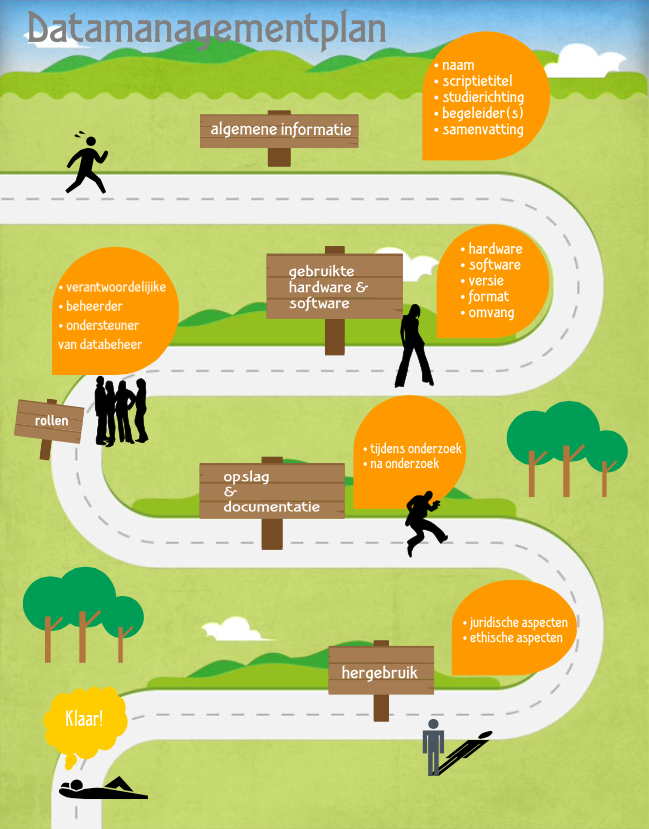
\includegraphics[width=0.6\textwidth]{img/dpm_studenten_infographic.png}
\caption{\label{fig:dmpinfo} \small Infographic voor het opstellen van een DMP. Gebaseerd op een werk van de Universiteitsbibliotheek Nijmegen op \href{http://ru.nl.libguides.com}{\textsf{http://ru.nl.libguides.com}}}
\end{center}
\end{figure}

In dit voorbeeld moet je een DMP opstellen voor een simpel onderzoek. In dit onderzoek worden fipronil-gehaltes bepaald in verschillende monsters. Fipronil is een schadelijke stof die een aantal jaren geleden in eieren terecht is gekomen, wat voor een landelijke herroeping van veel eieren heeft gezorgd. In dit onderzoek worden eieren van verschillende supermarkten onderzocht op fipronil-gehaltes. Het onderzoek wordt uitgevoerd bij het RIKILT (onderdeel van de Nederlandse voedsel- en warenautoriteit) door 2 studenten die daar stage lopen. 

Stap 1 in het DMP is het beschrijven van de algemene informatie:
\begin{table}[h]
\begin{tabular}{ll}
Onderzoekers    & H. van der Steeg, J. van der Maat                    \\
Titel onderzoek & Controleren van de gehaltes fipronil in supermarkteieren \\
Begeleiders     & Dr. B. Swennenhuis                                   \\
Bedrijf        & RIKILT Wageningen                                       \\
Datum      & 1/1/2020 tot 1/4/2020                                            
\end{tabular}
\end{table}

Nu moet er bedacht worden hoe de data wordt verkregen, opgeslagen, wie er verantwoordelijk is, etcetera.

\textbf{Details over het onderzoek}\\
Fipronil is een organisch molecuul wat wordt gemeten met behulp van een GC-MS. De ruwe data komt in .csv bestanden terecht en kan worden geanalyseerd met MSAnalyzer. De verwerkte data wordt opgeslagen als .xls bestand. De bestanden hebben een formaat van maximaal 1 MB per stuk (maar vaak een stuk kleiner). Er worden zo'n 100 eieren gemeten, en van ieder ei wordt zowel het eiwit als het eigeel doorgemeten in duplo. Alle ruwe data moet worden opgeslagen in verband met bewijslast. 

De MS wordt gebruikt om de fipronil-piek te identificeren en de hoogte van de piek in het chromatogram wordt gebruikt om het gehalte te bepalen. De uiteindelijk verwerkte uitkomsten van iedere meting (dus gehalte fipronil) zal in losse bestanden worden opgeslagen. 

De data wordt opgeslagen op de interne servers van het RIKILT. Hier kunnen alleen bevoegde medewerkers van het instituut bij. De bestanden moeten opgeslagen worden inclusief begeleidende tekst in het NL en EN die uitlegt wat er in de bestanden te vinden is en van welke sample de data afkomstig is. 

Er wordt verwacht dat de fipronilconcentratie onder de \SI[per-mode=symbol]{5}{\micro\gram\per\kilo\gram} ligt (maximaal toegestane waarde). Als de waardes hierboven liggen zal er direct melding van worden gemaakt bij de voedsel- en warenautoriteit in verband met een mogelijk gevaar voor de volksgezondheid. Bedrijven kunnen tot 5 jaar na overschrijding van maximale fipronilgehaltes een boete krijgen. 

\color{saxion}\textbf{Opdracht week 3: }\color{black} vul het sjabloon voor de DMP in voor deze case (zie appendix \ref{ap:dmp} of gebruik een ander sjabloon met een zelfde strekking), maak ook een voorbeeldmetadatabestand en mappenstructuur. Bewaar het gemaakte werk voor de eindopdracht.

\newpage
\section{Ordenen en opschonen van gegevens}
Als de gegevens uiteindelijk allemaal zijn verkregen is vaak de tweede stap om de data op te schonen, samen te voegen, en klaar te maken voor (semi-)langdurige opslag. Soms is dit heel simpel om te doen, maar vaak is dit een langduriger proces waarbij data uit verschillen bronnen en formats samengevoegd moeten worden tot een overzichtelijk geheel wat verder verwerkt kan worden.
Over het algemeen wordt hiervoor Excel gebruikt als softwarepakket. Met Excel kan je op veel verschillende manieren data importeren, inlezen, combineren, en weer opslaan in allerlei verschillende formats die door andere software kan worden ingelezen. In deze opleiding gebruiken we bijvoorbeeld R, SPSS, en Python om data verder te verwerken.

\color{saxion}\textbf{Opdracht week 4: }\color{black} Gebruik de kennis die je hebt vergaard de afgelopen 2 weken om een DMP te schrijven (en uit te voeren!) voor het project Chemical Fingerprinting. De data die je verzamelt voor het project ga je volgend kwartiel gebruiken voor een automatiseringsopdracht, dus het is van belang dat je de data op een goede manier opslaat!
\chapter{Multivariate data-analyse}
2 lessen: clusteranalyse en principale componentenanalyse

\section{Clusteranalyse}

\section{Principale-componentenanalyse}
\chapter{Gegevensbeheer}
2 lessen over databases


\chapter{Design of experiments}
doe dictaatje in R

\section{Wat is Design of Experiments?}
\section{Factorial Design}


\begin{appendices}
\backgroundsetup{contents={}}
\chapter{Handleiding multivariate data-analyse}
\label{app:multivariaat}

In deze appendix vind je een korte handleiding voor het uitvoeren van clusteranalyses en principale componentenanalyse met behulp van BlueSky en R. In de studiewijzer in dit document vind je de links om dit te installeren.

Onderstaande handleiding is een uittreksel van een groter dictaat, die is te vinden op Blackboard. In het dictaat staat de theoretische achtergrond van de methodes. In dit uittreksel is alleen de handleiding voor het uitvoeren en deels voor het interpreteren van de data opgenomen, inclusief oefenopdrachten.

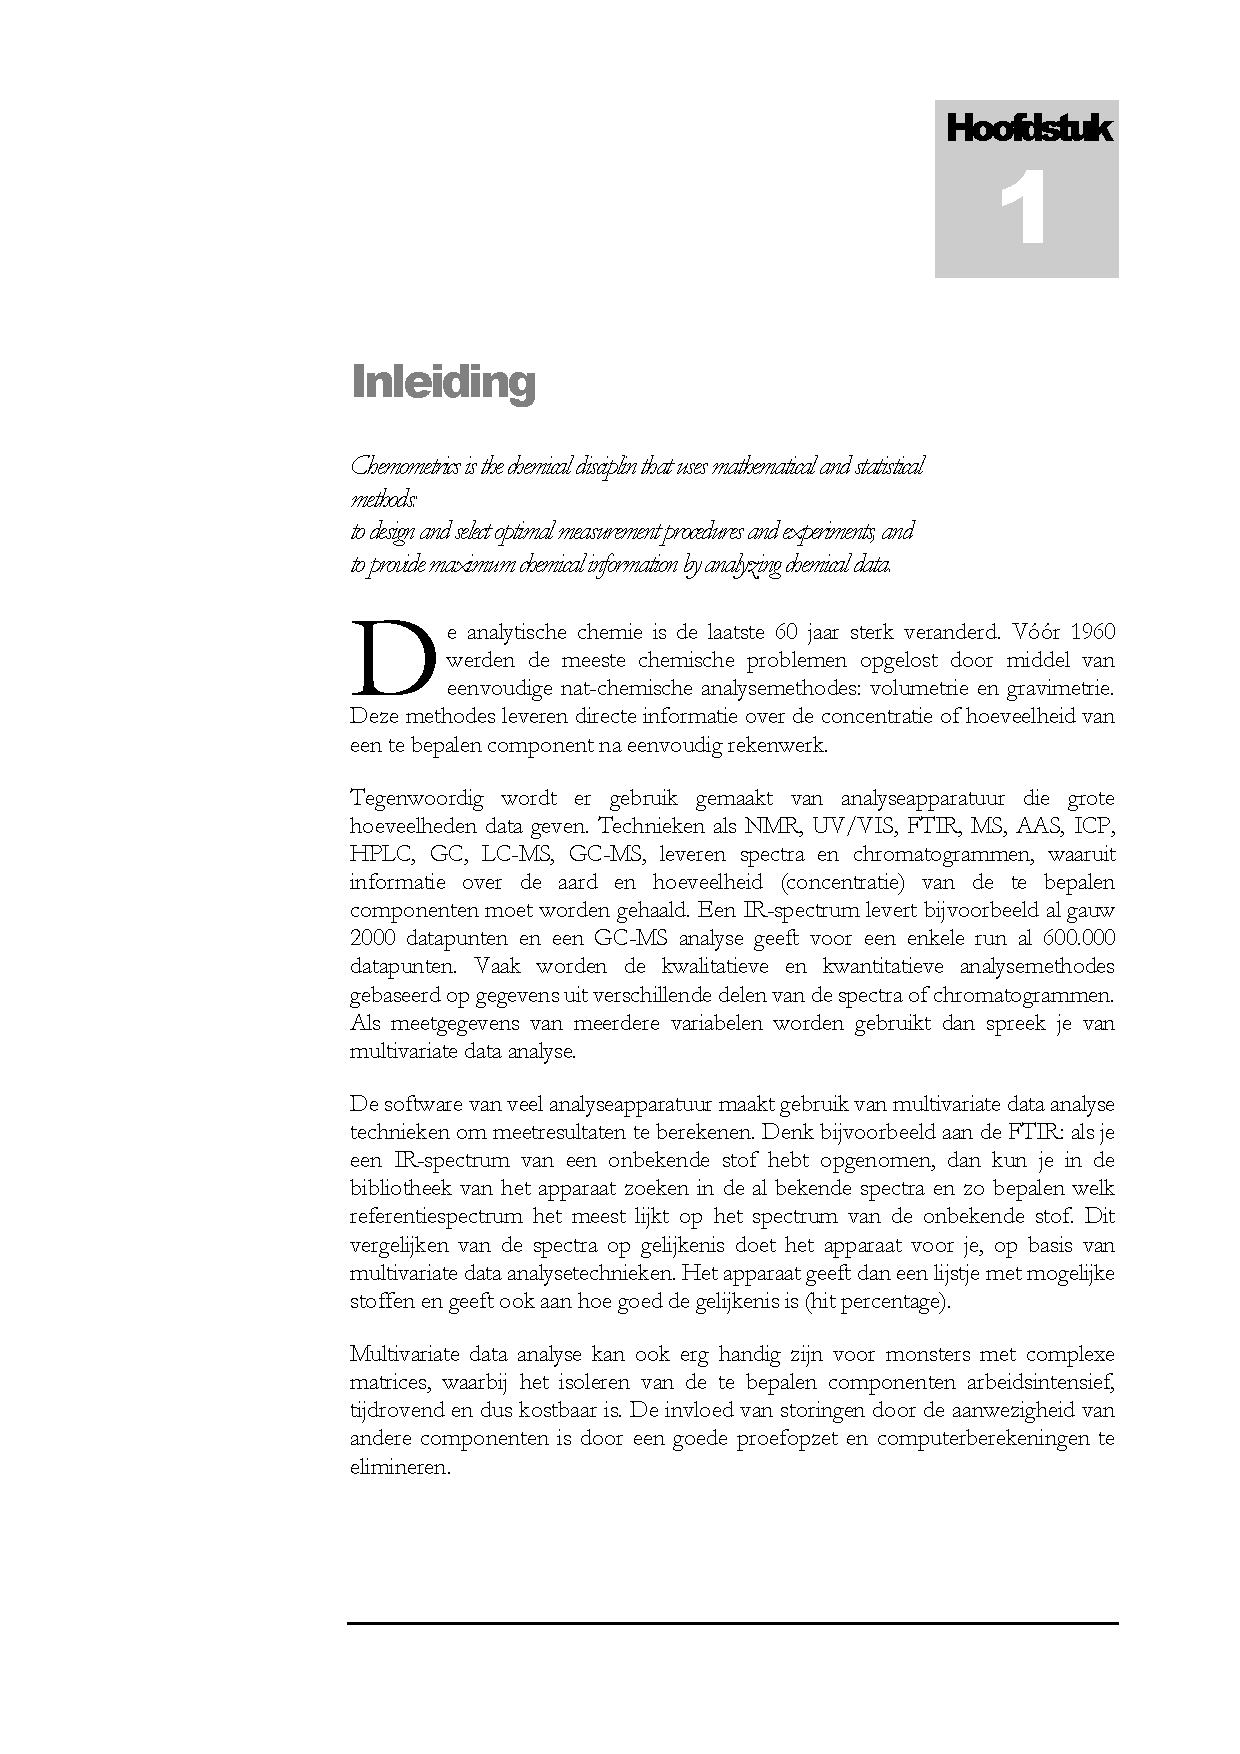
\includepdf[pages=-, nup=2x2]{img/multivariaat.pdf}
\chapter{Sjabloon DMP}
\label{ap:dmp}
Onderstaand sjabloon voor het maken van een DMP kan je gebruiken voor je projecten. Je mag dit uiteraard ook aanpassen indien nodig. Dit sjabloon is verkregen van de \href{https://libguides.ru.nl/datamanagement/dm}{\textsf{universiteitsbibliotheek van de Radboud Universiteit}}. Via die link vind je ook nog wat extra informatie en voorbeelden. 

Gebaseerd op een werk van de Universiteitsbibliotheek Nijmegen op \href{http://ru.nl.libguides.com}{\textsf{http://ru.nl.libguides.com}}
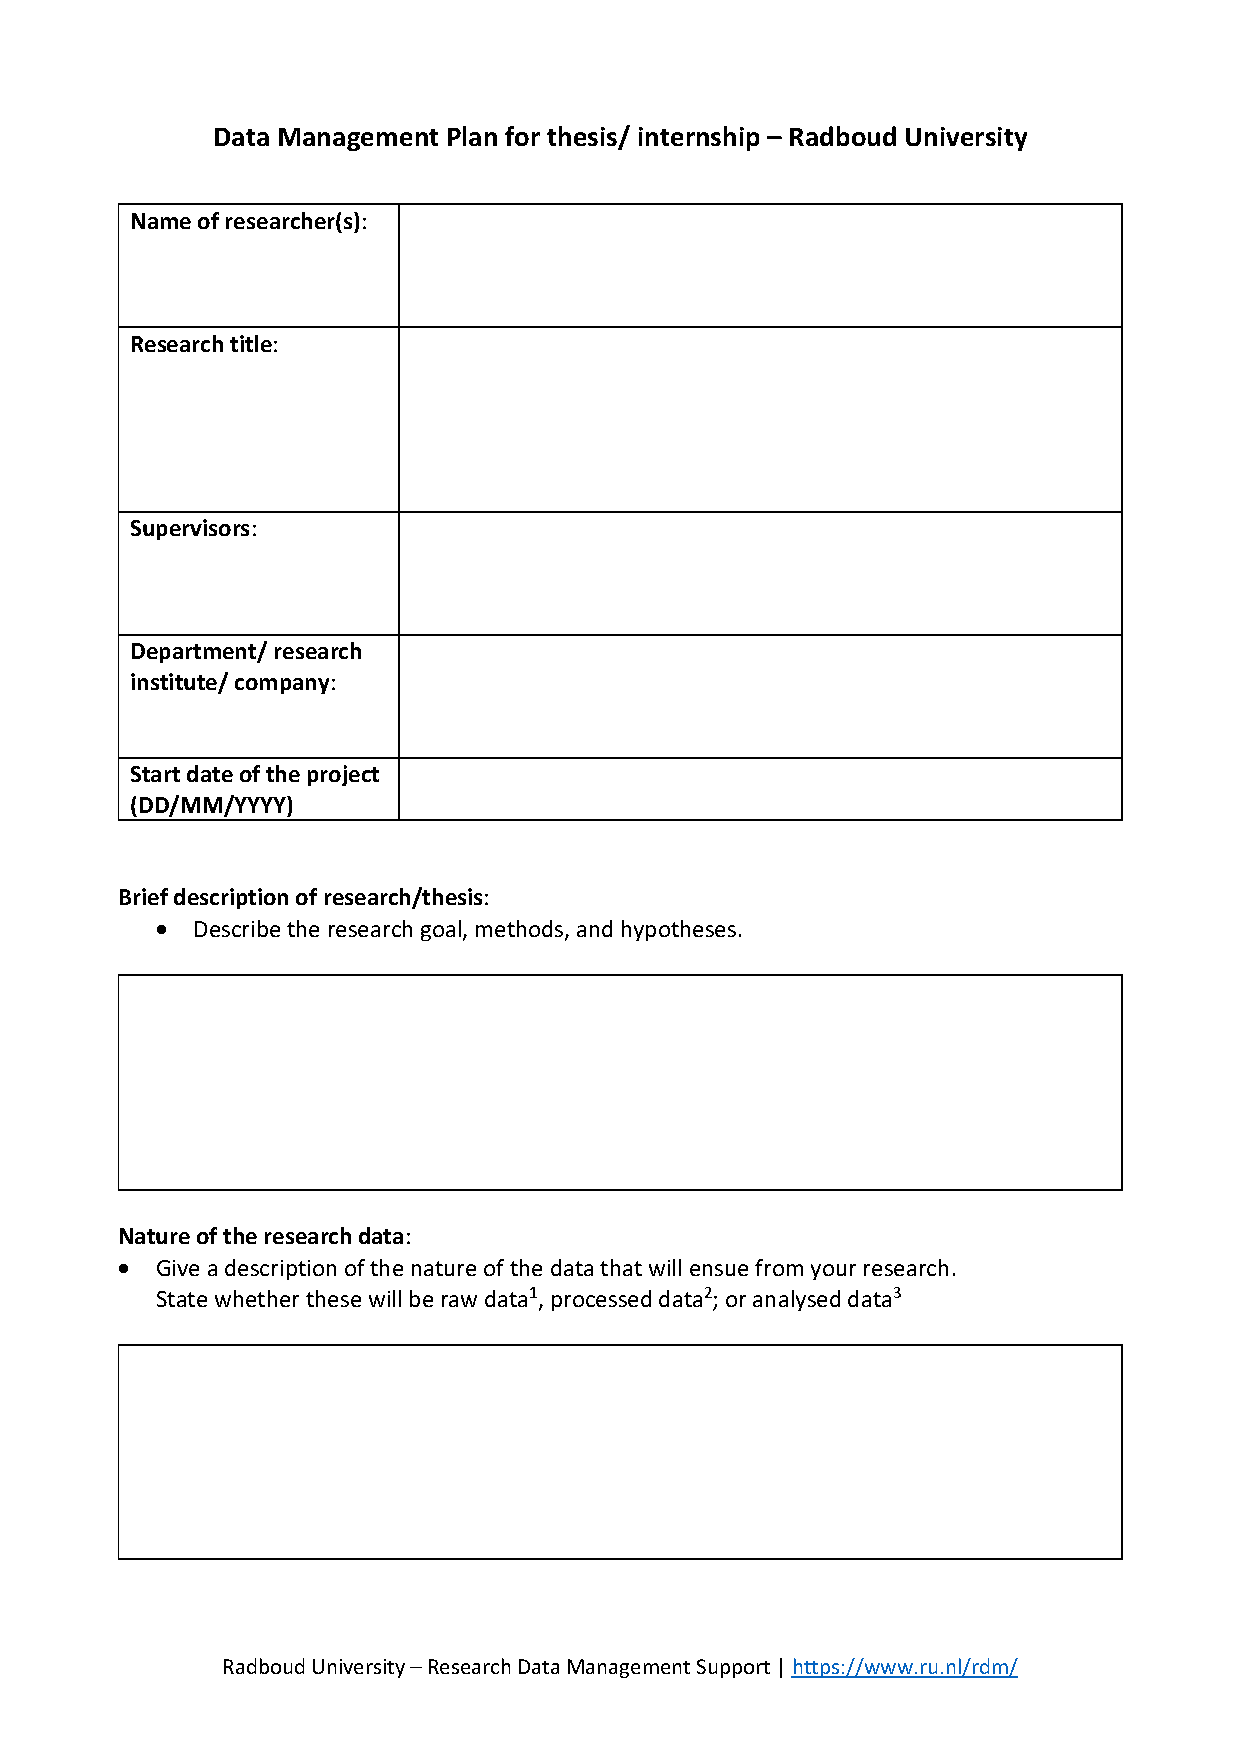
\includepdf[pages=-, nup=2x2]{dmp.pdf}

\end{appendices}

\end{document}
